
\subsection{Introducción}


<<<<<<< HEAD
\subsubsection{Introducción}
El conversor sigma-delta o delta-sigma según la literatura consultada, tuvo su aparición durante los años 60's y 70's. Aunque su nombre pueda sugerir un tipo de tecnología muy compleja la realidad es que no lo es en términos constructivos. Los moduladores sigma-delta nos permiten alcanzar una digitalización de alta resolución (16bits o 24bits) sin la necesidad de utilizar ADC de ese porte. Esto se consigue dado que este diseño permite alcanzar un nivel de ruido de cuantización equivalente a la de un ADC de mayor porte utilizando un ADC más modesto.
El modulador sigma-delta se vale de los beneficios del oversampling para conseguir un diseño sencillo y eficaz.
Un componente que esta presente en todos los ADC es el FAA, filtro anti-alias, que se coloca a la entrada del ADC para evitar solapamientos espectrales cuando se realiza el muestreo interno. En el caso del sigma-delta,  la señal es sobre muestreada por más de 64 por sobre la frecuencia de nyquist. Esto implica que las replicas del espectro de banda base se encontraran más alejada entre sí en el espectro.
\begin{figure}[H]
	\centering
	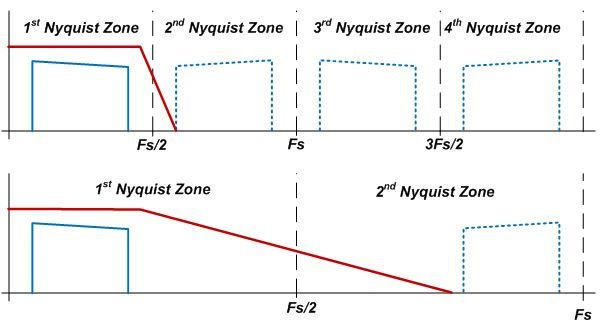
\includegraphics[width=0.7\linewidth]{ImagenesEjercicio2/Oversampling}
	\caption{Efectos del oversampling sobre las replicas espectrales}
	\label{fig:oversampling}
\end{figure}
Esto nos permite utilizar un filtro anti-alias de bajo orden, los cuales son más sencillos de realizar.


Además como se vera en secciones posteriores, el sobre-muestreo mejorara notablemente la performance de nuestro sencillo ADC de un 1-bit.

\subsubsection{Arquitectura}
=======
\subsection{Arquitectura}
>>>>>>> 67435597220b151a8b5cda66c526e8121bdc0398

A continuación presentamos la topología implementada:

\begin{figure}[H]
	\centering
	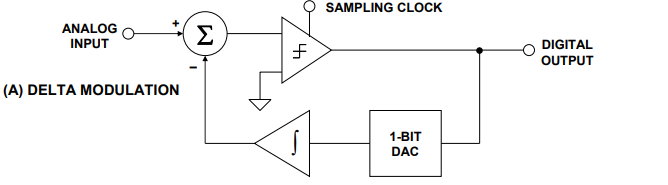
\includegraphics[width=0.7\linewidth]{ImagenesEjercicio2/diagramaEnBloques}
	\caption{Modulador $\Sigma\Delta$ de primer orden}
	\label{fig:diagramaenbloques}
\end{figure}

Como se puede observar el modulador $\Sigma\Delta$ se basa en un circuito con un solo camino de realimentación negativa que incorpora un cuantificador y un DAC en su interior.

El input analógico ingresa al sistema y se determina si el valor de la señal en ese instante es mayor o menor que su valor anterior. De esta forma conseguimos traducir la información analogica a un código binario que representa la señal en términos de los cambios en la señal.



<<<<<<< HEAD
\subsubsection{Modulador}
La salida del modulador $\Sigma\Delta$ es un bit-stream de valores binarios unipolares o bipolares, acorde al diseño utilizado. En esta secuencia se encuentra codificada toda la información necesaria para poder reconstruir la señal original. Aún más importante que reconstruir la señal original, es conseguir un valor preciso de la misma en un instante de tiempo. Es decir, poder tomar mediciones. Este tipo de conversores son famosos por la alta resolución que son capaces de proveer. Sin embargo, el limite de su funcionalidad aparece cuando se los quiere utilizar en un ambiente donde la señales cambian de forma abrupta.
=======
\subsection{Modulador}
La salida del modulador $\Sigma\Delta$ es un bit-stream de valores binario arbitrarios. En esta secuencia se encuentra codificada toda la información necesaria para poder reconstruir la señal original. Aún más importante que reconstruir la señal original, es conseguir un valor preciso de la misma en un instante de tiempo. Es decir, poder tomar mediciones. Este tipo de conversores son famosos por la alta resolución que son capaces de proveer. Sin embargo, el limite de su funcionalidad aparece cuando se los quiere utilizar en un ambiente donde la señales cambian de forma abrupta.
>>>>>>> 67435597220b151a8b5cda66c526e8121bdc0398

\begin{figure}[H]
	\centering
	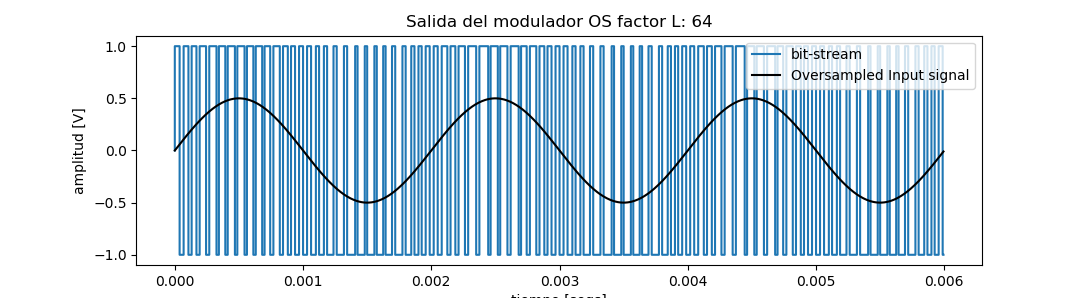
\includegraphics[width=0.7\linewidth]{ImagenesEjercicio2/BitsStream64}
	\caption{}
	\label{fig:bitsstream64}
\end{figure}


\subsection{Noise Shaping}
Una de las más notables características de este tipo de modulación es el efecto llamado \textbf{noise-shaping}. Este efecto provoca que el ruido de cuantización sea "moldeado" hacia las altas frecuencias empujándolo lejos de la banda de interés.


\begin{figure}[H]
	\centering
	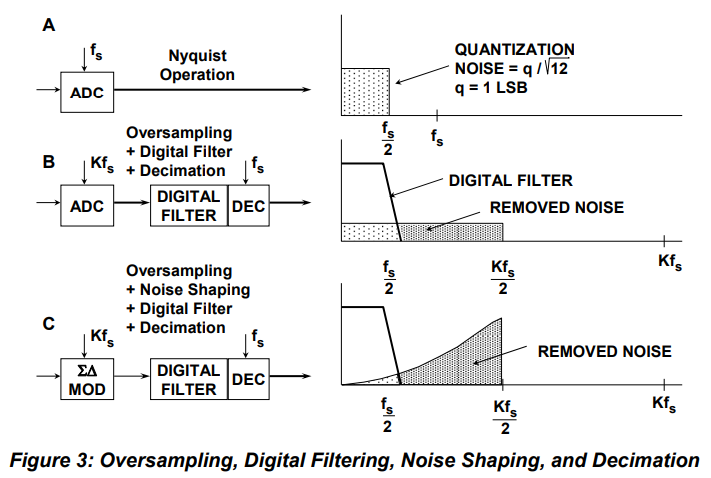
\includegraphics[width=0.7\linewidth]{ImagenesEjercicio2/NoiseShappingAN}
	\caption{}
	\label{fig:noiseshappingan}
\end{figure}


Esto implica que el ruido de cuantización efectivo, dentro de la banda de interés, se ve reducido. Esto es equivalente a pensar que la señal fue cuantizada mediante un cuantizador que tiene un ruido de cuantización proporcional al ruido restante sobre la banda de interés.

En la siguiente imagen vemos la salida del modulador, podemos elegir entre salida unipolar o monopolar dependiendo de como se realice el post-procesamiento que se le de luego de la modulación.
 
\begin{figure}[H]
	\centering
	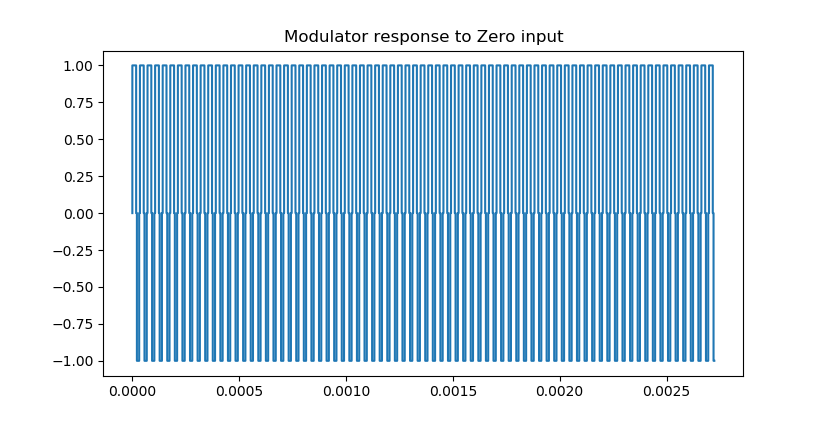
\includegraphics[width=0.7\linewidth]{ImagenesEjercicio2/OutoutZeroInput}
	\caption{Salida del modulador con Input nulo}
	\label{fig:outoutzeroinput}
\end{figure}

Podemos observar como al usar un gran frecuencia de sampleo obtenemos la caracteristica curva de noise-shaping del ruido de cuantización.
\begin{figure}[H]
	\centering
	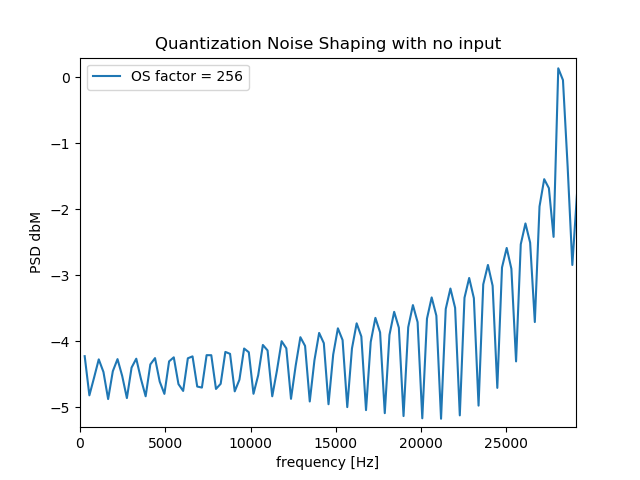
\includegraphics[width=0.7\linewidth]{ImagenesEjercicio2/QnoiseNoInput}
	\caption{}
	\label{fig:qnoisenoinput}
\end{figure}


A continuación aplicamos la modulación sigma-delta sobre una señal senoidal con una frecuencia fundamental de $500Hz$. 
\begin{figure}[H]
	\centering
	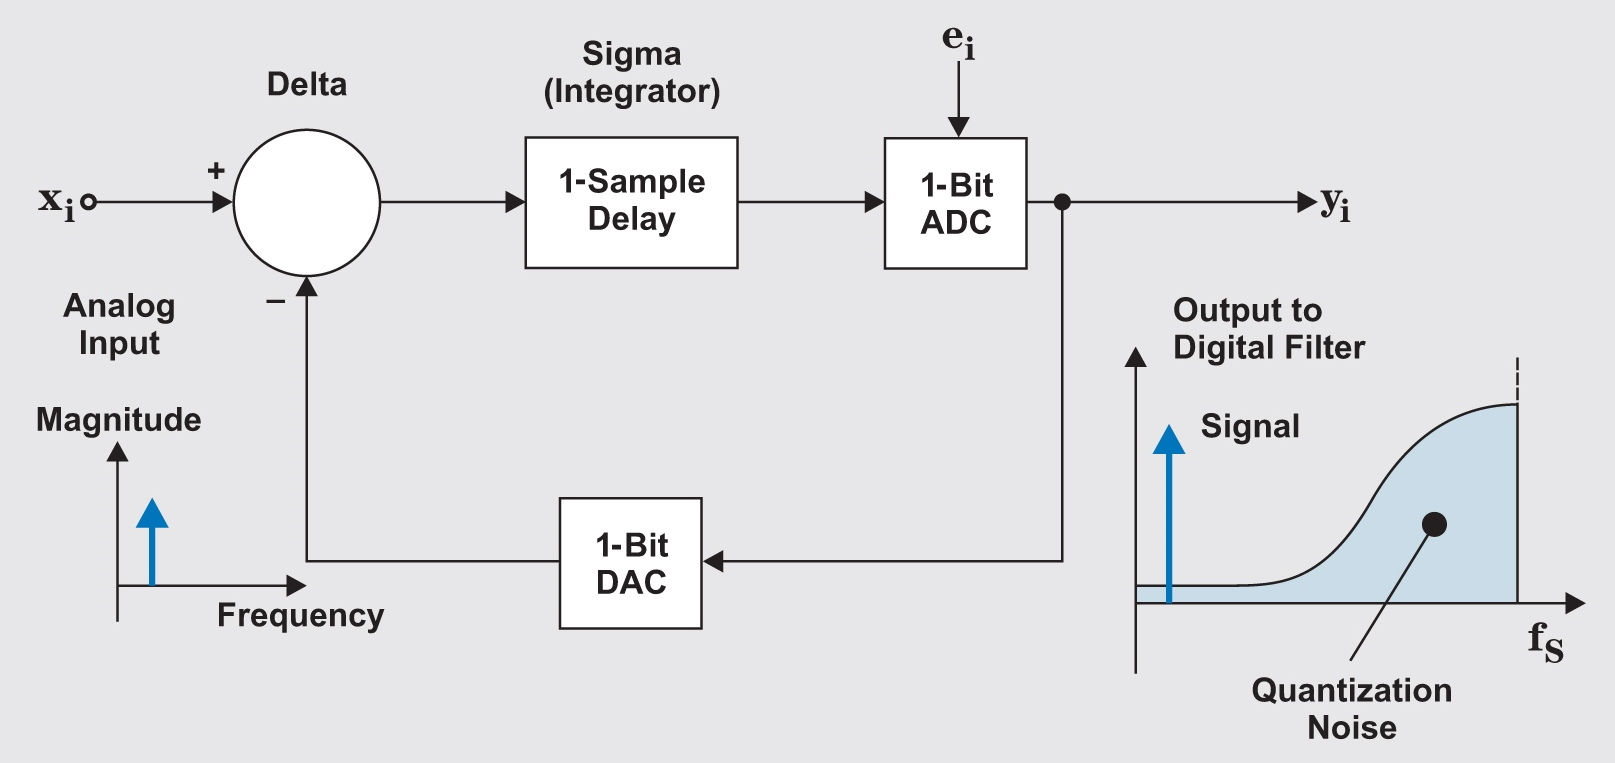
\includegraphics[width=0.7\linewidth]{ImagenesEjercicio2/NoiseShapingFullsche}
	\caption{}
	\label{fig:noiseshapingfullsche}
\end{figure}



Debajo muestran los resultados obtenidos luego de realizar el periodograma sobre los bits de salida

\begin{figure}[H]
	\centering
	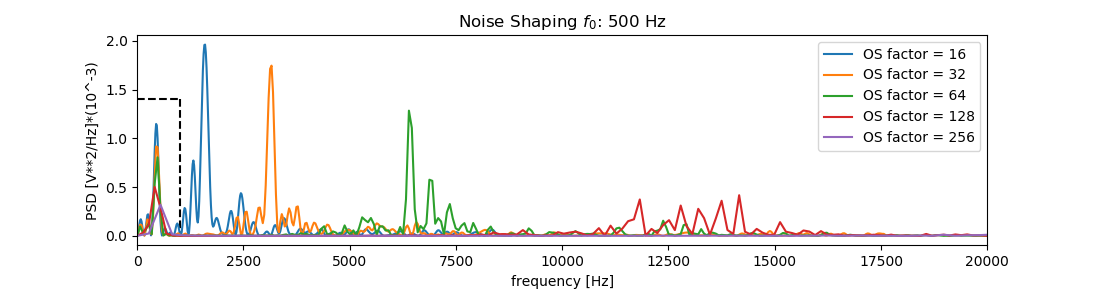
\includegraphics[width=\linewidth]{ImagenesEjercicio2/NoiseShappingDemo1zoom2solid.png}
	\caption{Noise Shapping con diferentes niveles de sobremuestreo}
	\label{fig:noiseshappingdemo1}
\end{figure}
En primer lugar podemos ver que a medida que aumentamos la tasa de oversampling (OS), el ruido de cuantización se aleja más de la banda de interés e incursiona hacia posiciones más elevadas en el espectro.

\begin{figure}[H]
	\centering
	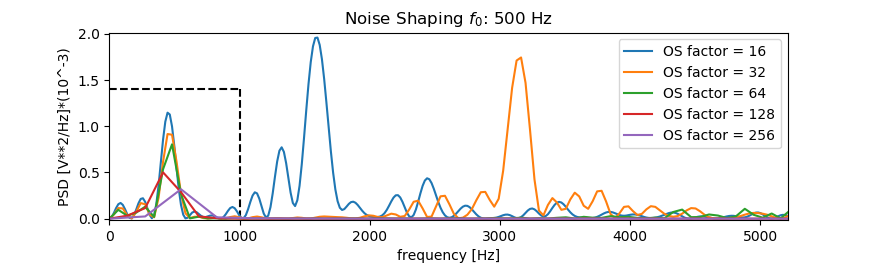
\includegraphics[width=\linewidth]{ImagenesEjercicio2/NoiseShappingSolidZoom.png}
	\caption{Noise Shapping con diferentes niveles de sobremuestreo, acercamiento}
	\label{fig:noiseshappingdemo1}
\end{figure}

Si reescalamos la potencia espectral y la expresamos en dBm conseguimos apreciar notoriamente el noise-shapping.

El pico observado a bajas frecuencias corresponde a la frecuencia fundamental de nuestra información de entrada
\begin{figure}[H]
	\centering
	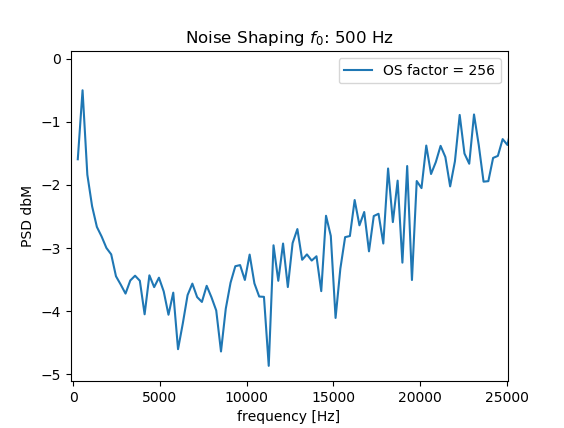
\includegraphics[scale=0.7]{ImagenesEjercicio2/NoiseShappingdbM.png}
	\caption{Noise Shapping}
	\label{fig:noiseshappingdemo1}
\end{figure}
<<<<<<< HEAD

\subsubsection{Decimación}
El objetivo de sobremuestrear la señal era el de aumentar la resolución de nuestro ADC. Sin embargo, la tasa de información generada puede ser demasiado alta como para que la circuiteria posterior pueda manejarla de manera efectiva. Es por eso que luego del proceso de modulación se filtra la señal de salida y se reduce la cantidad de muestras de la misma.

Debajo se pueden ver diversos experimentos realizados.

\begin{figure}[H]
	\centering
	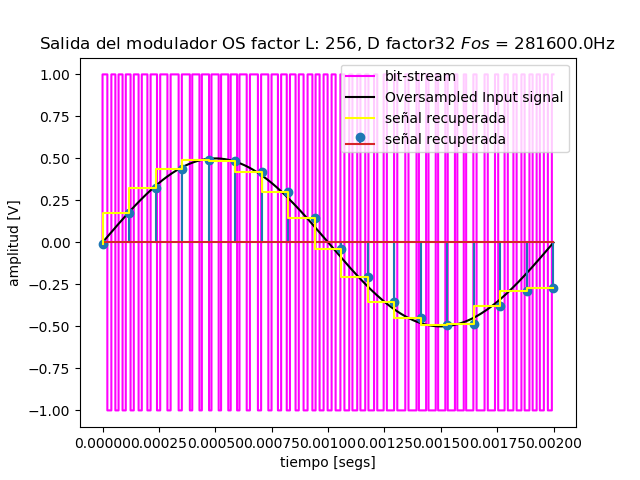
\includegraphics[width=0.7\linewidth]{ImagenesEjercicio2/SenalRecuperada256.png}
	\caption{}
	\label{fig:senalrecuperada256}
\end{figure}
\begin{figure}[H]
	\centering
	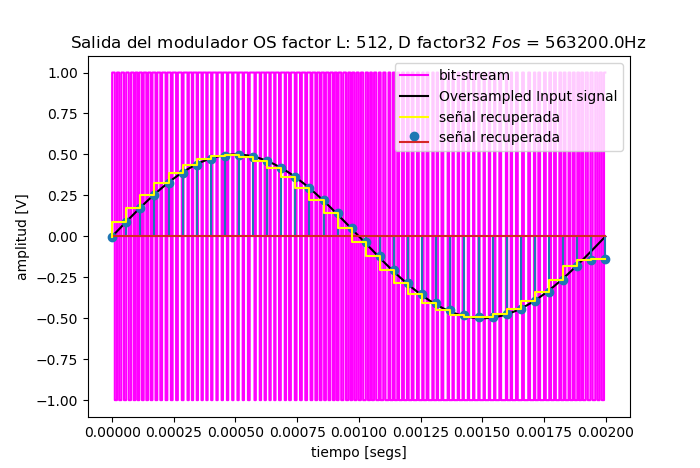
\includegraphics[width=0.7\linewidth]{ImagenesEjercicio2/SenalRecuperada512.png}
	\caption{}
	\label{fig:senalrecuperada256}
\end{figure}

\subsubsection{Simulaciones}
Se realizaron las simulaciones íntegramente en Python, se recomienda correr el archivo \textbf{demos.py} para ver todas las demostraciones.

\end{document}
=======
>>>>>>> 67435597220b151a8b5cda66c526e8121bdc0398
